\documentclass{article}
\usepackage[utf8]{inputenc}
\usepackage{graphicx}
\usepackage{geometry}
\usepackage{hyperref}
\hypersetup{
    colorlinks,
    citecolor=black,
    filecolor=black,
    linkcolor=black,
    urlcolor=black
}

 \geometry{
 a4paper,
 left=30mm,
 right=30mm,
 top=30mm,
 }

\graphicspath{ {Images/} }

%----------------------------------------------------------------------------------------
%	TITLE PAGE
%----------------------------------------------------------------------------------------

\newcommand*{\titleGP}{\begingroup
		\begin{figure}[t]
			\centering
			
\includegraphics[width=350px]{UP_Logo.PNG}
		\end{figure}
\centering 
\vspace*{\baselineskip}

\rule{\textwidth}{1.6pt}\vspace*{-\baselineskip}\vspace*{2pt}
\rule{\textwidth}{0.4pt}\\[\baselineskip]

{\LARGE NavUP\\ [0.3\baselineskip] Longsword Testing Report on Broadsword Data } \\ [0.2\baselineskip]
\rule{\textwidth}{0.4pt}\vspace*{-\baselineskip}\vspace{3.2pt}
\rule{\textwidth}{1.6pt}\\[\baselineskip] %

% \scshape %
% A concise specification on the functional requirements  \\
% and use cases of NavUP \\[\baselineskip]

% \vspace*{2\baselineskip}

Compiled By \\[\baselineskip]
{\Large Lucian Sargeant - u15225560 \\ Ritesh Doolabh - u15075754 \\ Peter Boxall -  u14056136 \\ Claude Greeff - u13153740\\ Harris Leshaba - u15312144 \\ Hristian Vitrychenko - u15006442\par}

\bigskip
\bigskip

 	GitHub Repository:  
 	\href{https://github.com/Chris19951225/COS-301-Longsword-Data-Streaming}{COS 301 Team Longsword Data GitHub Repository(Phase 4)}
\\
 	Slack Group:  
 	\href{https://cos301longsworddata.slack.com/messages/C4JMSNZGE/}{COS 301 Team Longsword Data Slack Group(Phase 4)}
 	\\
 	Scrum-board:  
 	\href{https://waffle.io/Chris19951225/COS-301-Longsword-Data-Streaming}{COS 301 Team Longsword Data Scrum-board(Phase 4)}
 	\\
 	Burn-down Chart:  
 	\href{https://waffle.io/Chris19951225/COS-301-Longsword-Data-Streaming/metrics/burndown?milestone=Testing\%20Phase\%20Deadline}{COS 301 Team Longsword Data Burn-down Chart(Phase 4)}




 

\vfill


{\scshape 2017} \\[0.3\baselineskip]
{\large TEAM LONGSWORD (DATA)}\par

\endgroup}

\begin{document}

\titleGP
\newpage
\tableofcontents

\newpage

\section{Introduction}
\begin{flushleft}
For this phase we will be testing the Data module of the BroadSword Team. We have split the testing phase according to Functional Requirements, Non-Functional Requirements, Use Cases and Testing Cases. 
\end{flushleft}

\begin{flushleft}
Their code was primarily coded in Python and used a NSQ message processing system.
We will be testing the various cases and giving a brief description of how we tested followed by an explanation of the mark that was given to them.
\end{flushleft}

\section{Testing Methods}
\begin{flushleft}
The testing of the Data module becomes more complex due to the fact that multiple independent components are used to achieve the purpose of data streaming. This then means that we had to integrate code within the files given us so that we could effectively and accurately test the system given to us. With the regard to the aforementioned, it can be clearly seen that the use of any form of a unit testing framework would be difficult to implement and thus we opted for the integrated code test. This form of testing also shows which part/s of the code given to us performed its actions to the necessary pedigree and which part/s did not.
\end{flushleft}

\newpage
\section{Service Contracts}

\subsection{Retrieving and passing device MAC address.}
\begin{flushleft}
MARK: 10
\end{flushleft}

\begin{flushleft}
The access module sends a location request to the data module via the NSQ server,the access module has to subscribes to a topic.The main entry point of the system, query resolver.py, sends the mac address to the Aruba server in a query to get the location of the device.
In query resolver.py, the handler function receives a request, it then passes the mac address to the searcher function-which will create a query to get the location for the device.
\end{flushleft}

\begin{flushleft}
This functional requirement was fulfilled by the Broadsword team.
\end{flushleft}
\begin{figure}[ht]
  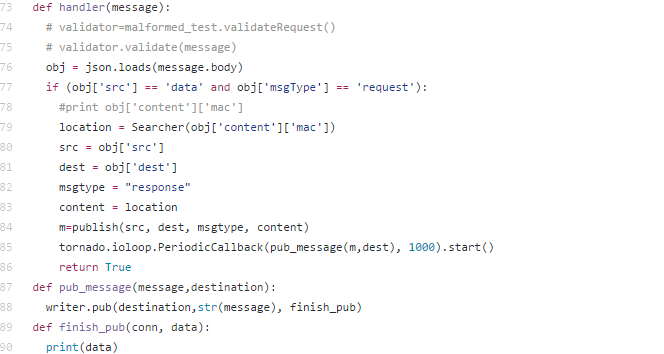
\includegraphics[width=350px]{Handler.png}

\caption{Handler function.}
  \label{Handler function}
\end{figure}

\subsection{Logging in and maintaining a session with Aruba ALE.}

\begin{flushleft}
MARK: 4
\end{flushleft}

\begin{flushleft}
The Broadsword data team does indeed log in to the Aruba ALE and they do this by making use of the python urllib2 library. Their query\textunderscore resolver.py entry point takes arguments for the various ALE login fields, the arguments are passed between classes until reaching the Aruba class which is instantiated with the details. This Aruba class contains a method called get() which effectively creates a URL, containing the address for accessing Aruba appended by the current request. The login is then handled with a password manager and finally the function returns the JSON formatted response from Aruba. The function can be seen in the figure below.
\end{flushleft}

\newpage
\begin{figure}[ht]
  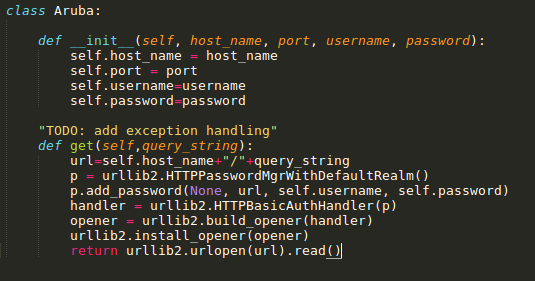
\includegraphics[width=350px]{Images/Get_Function.png}
  \caption{Implementation of the Aruba Wrapper class.}
  \label{get() function.}
\end{figure}

\begin{flushleft}
There is however a grave issue with this approach as each time the get() function is called, which occurs for every request, the login to Aruba needs to happen again as a session is not maintained. This results in a massive time overhead especially considering that the program is intended to be scaled to handle tens of thousands of requests a second. This is simply not possible with Broadswords code as it stands, as each request-response pair to Aruba is taking roughly a second to complete. This can been seen in the diagram below where only 73 requests were processed in a minute.
\end{flushleft}

\begin{figure}[ht]
  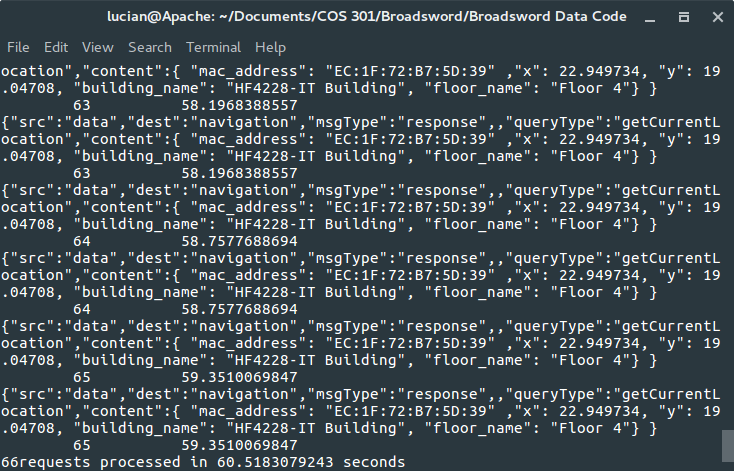
\includegraphics[width=350px]{Images/Aruba_Returns.png}
  \caption{The number of Aruba requests processed in one minute.}
  \label{Terminal output.}
\end{figure}



\newpage
\subsection{Processing the request and retrieving location.}

\begin{flushleft}
MARK: 10
\end{flushleft}

\begin{flushleft}
In the python file query\textunderscore resolver.py, Broadsword provides the options of using mock data to test their program or to follow standard procedure and use real data from Aruba by connecting to it through location\textunderscore lookup.py, building\textunderscore lookup.py and floor\textunderscore lookup.py. The previously mentioned python files each connect to Aruba and all separately log in by utilising Aruba\textunderscore wrapper.py which establishes and maintains a session with Aruba. Each class also filters their own JSON objects that are returned by Aruba and return only the necessary data thus fulfilling the requirement of processing requests and retrieving location. 
\end{flushleft}
  
\begin{flushleft}
This functional requirement was not fully fulfilled by the Broadsword team.
\end{flushleft}

\begin{figure}[ht]
  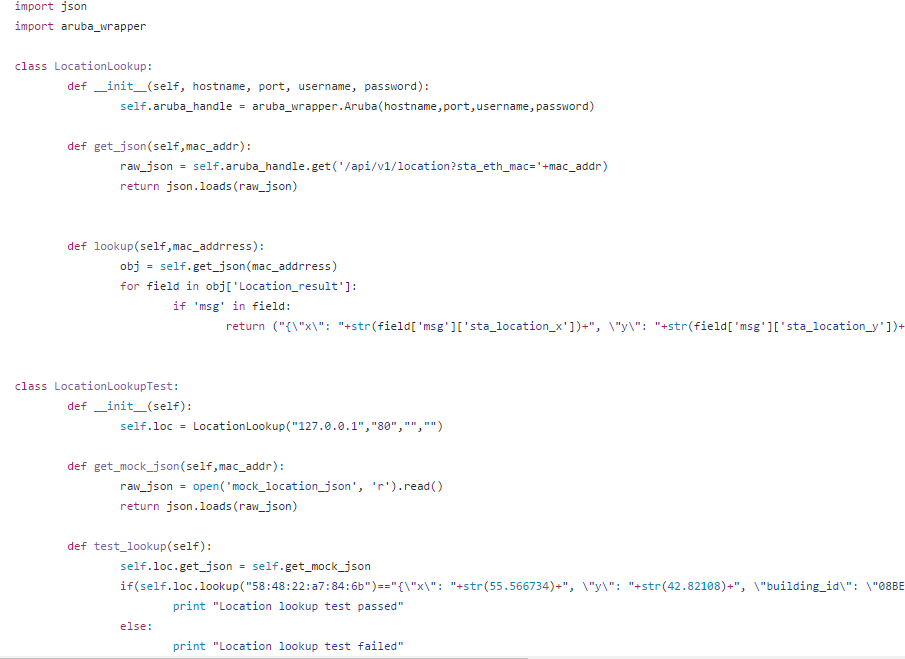
\includegraphics[width=350px]{Images/getLoc.PNG}
  \caption{Aruba\textunderscore wrapper.py}
  \label{arubawrapper.py}
\end{figure}
\newpage
\begin{figure}[ht]
  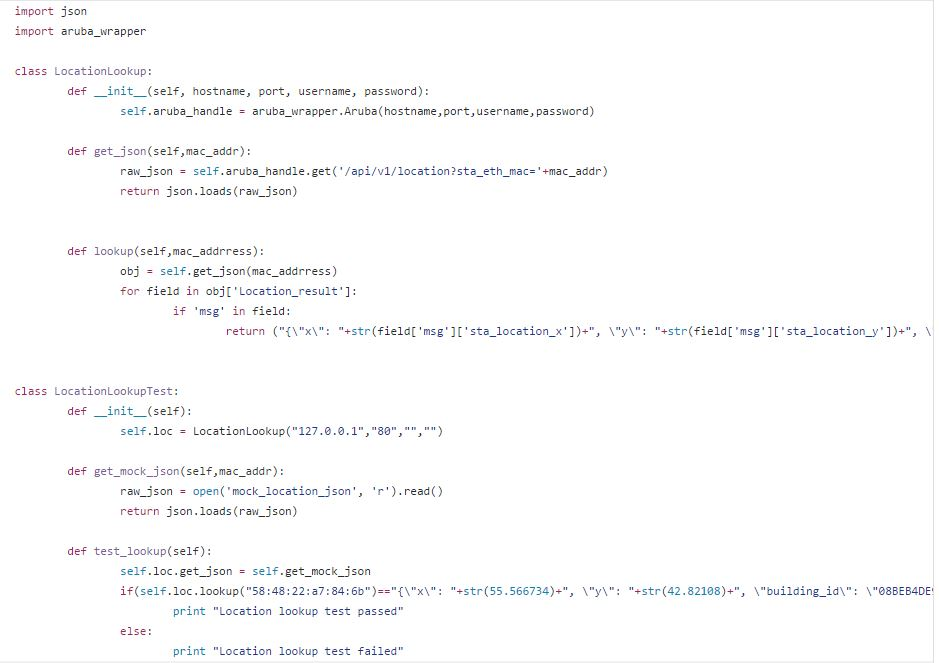
\includegraphics[width=350px]{Images/LocLookup.JPG}
  \caption{Mock JSON}

\label{Mock JSON}
\end{figure}


\subsection{Returning a location to the source of the request.}
\begin{flushleft}
MARK: 8
\end{flushleft}

\begin{flushleft}
After the Aruba ALE connection is made by the Aruba-wrapper class, the results of the location query are then delt with in the LocationLookup class. This class instantiates and executes the Aruba-wrapper implementation and then processes the JSON results to filter out what is needed. 
\end{flushleft}

\begin{flushleft}
This functional requirement was fulfilled by the Broadsword team.
\end{flushleft}

\begin{figure}[ht]
  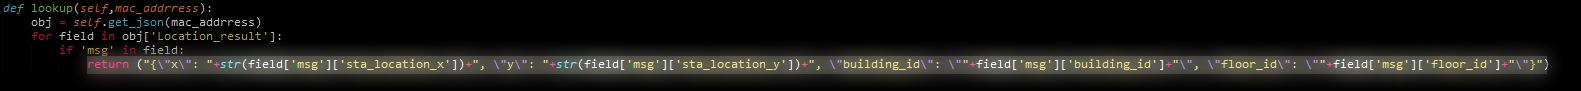
\includegraphics[width=350px]{Images/jsonreturn.jpg}
  \caption{JSON returned}
  \label{fig:JSON returned}
\end{figure}

\newpage
\section{Non-Functional Requirements}

\subsection{Level of concurrency of the task.}
\begin{flushleft}
MARK: 0
\end{flushleft}

\begin{flushleft}
Broadsword made use of a server known as NSQ which is widely known for its message passing based procedures. Whilst the NSQ core was built in Go (a programming language with built in concurrent), Broadsword did not seem to make use of any of those concurrent features in their code. This was made apparent in testNavigationConsumer.py where each NSQ action was made on after the other with no concurrency apparent anywhere in terms of mac address processing and message passing. In terms of concurrent programming in general, there is none in any of the code presented by Broadsword. 
\end{flushleft}

\begin{flushleft}
This non-functional requirement was not fulfilled by the Broadsword team.
\end{flushleft}

\begin{figure}[ht]
  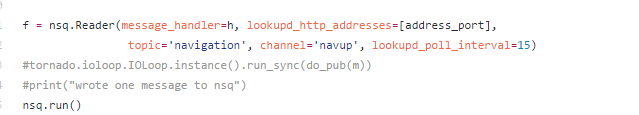
\includegraphics[width=350px]{Images/concurrency.PNG}
  \caption{NSQ Use Without Concurrency}
  \label{NSQ Use Without Concurrency}
\end{figure}

\begin{figure}[ht]
  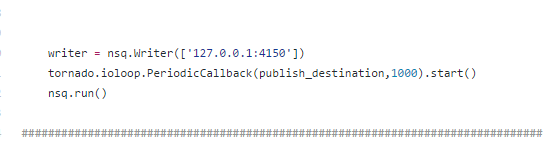
\includegraphics[width=350px]{Images/concurrency2.PNG}
  \caption{NSQ Writer}
  \label{NSQ Writer}
\end{figure}

\subsection{Performance of the request processing.}
\begin{flushleft}
MARK: 2
\end{flushleft}

\begin{flushleft}
Broadsword used a NSQ server which is a message passing system that primarily relies on queue structures to store information. Although NSQ does allow for concurrent programmability, these features were not used efficiently enough to allow large numbers of requests to be "streamed" at high speeds. We simply used a timer in their code to count the number of instances of the location object that was returned for a specific MAC address. This terminated the code after 60 seconds and gave the final number of instances returned.   
\end{flushleft}

\begin{flushleft}
As can be seen from the screen-shots below, within the duration of 60 seconds, the system only managed to return 73 Location objects for a single mac address. In terms of real-world functionality, this would mean a significant bottleneck on the system. This is because the system would need at a minimum roughly 30 000 requests to be fulfilled in a matter of 60 seconds. In the regard of high speed data streaming, the Broadsword Data module has failed.
\end{flushleft}

\begin{flushleft}
This non-functional requirement was not fulfilled by the Broadsword team.
\end{flushleft}

\begin{figure}[ht]
  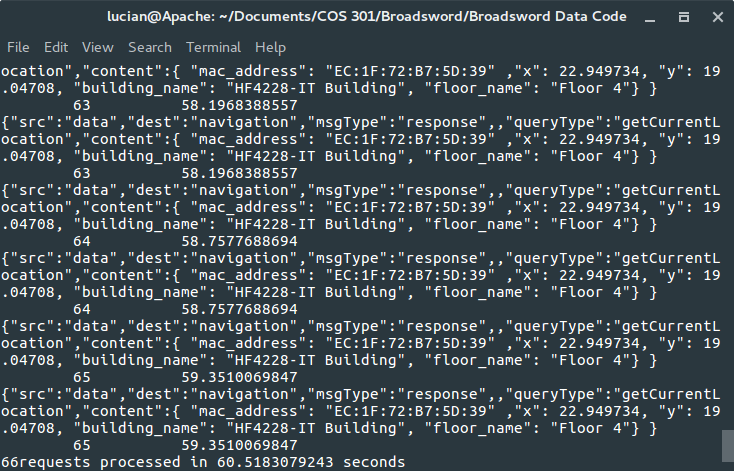
\includegraphics[width=350px]{Images/Aruba_Returns.png}
  \caption{Number of requests processed in 60 Seconds}
  \label{Number of Requests}
\end{figure}
\newpage
\begin{figure}[ht]
  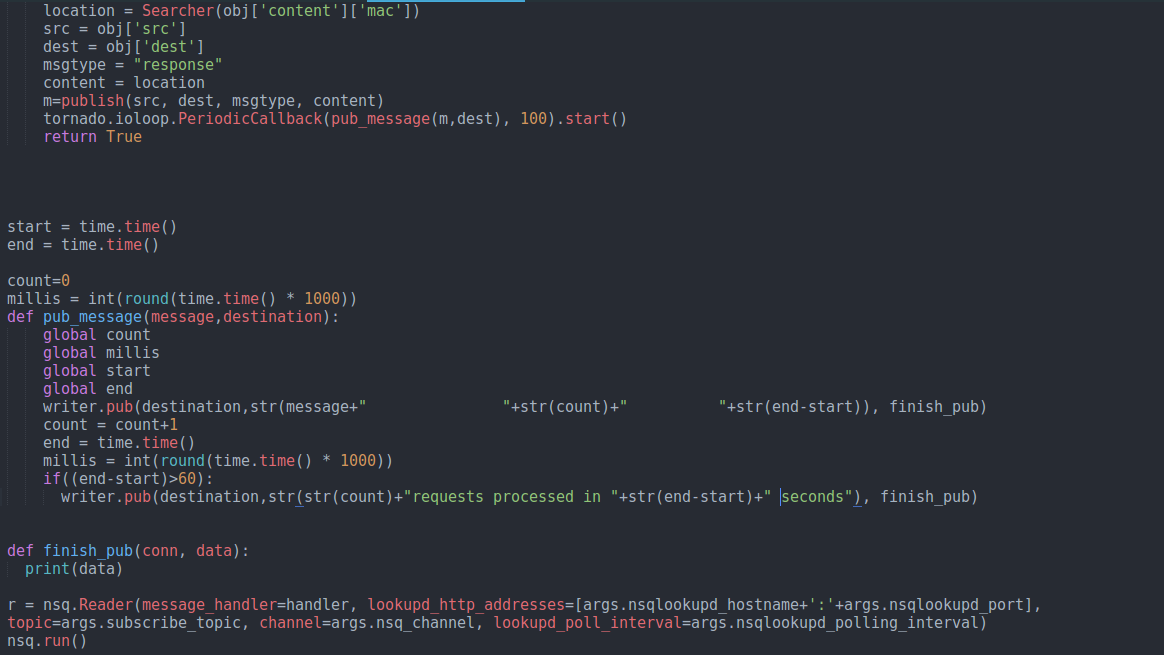
\includegraphics[width=350px]{Images/timer.png}
  \caption{Code inserted to test the number of requests processed in 60 seconds}
  \label{Testing Code}

\end{figure}

\newpage
\subsection{Maintainability and modularity of the code and repository.}

\begin{flushleft}
MARK: 4
\end{flushleft}

\begin{flushleft}
For someone not intimately familiar with the code, it is fairly difficult to understand the flow of the program. There is decent documentation on getting the code operational however the explanation of how the program actually works is lacking and to make matters worse there are also no comments in the code to explain what is happening. This could make maintaining the code an issue as if the developers need to return to it after a long time even they may have issues remembering exactly how the program flows and functions.
\end{flushleft}

\begin{flushleft}
The code is very modular having been separated effectively into separate classes based on function, which is good however once again it makes the program difficult to follow without any commenting.
\end{flushleft}

\begin{flushleft}
Finally, the GitHub repository is disorganised. It has been divided into a number of branches that do each each have an explained function however, as the repository stands, the branches are unsynchronised and not fulfilling their intended function.
\end{flushleft}

\begin{flushleft}
All of the above considered Broadsword receives the mark of 4/10 for this section.
\end{flushleft}


\subsection{Integrability and ease of transfer into a final system.}
\begin{flushleft}
MARK: 5
\end{flushleft}

\begin{flushleft}
Whilst the code is very modular in format allowing for certain pieces to be easily matched to other systems, the code appears to be fragmented to a stage where there are a lot of inter-dependency between these classes. Meaning It would be harder to break the system up and mould it to a new system. Also the lack of commenting makes it difficult for one to see where things are implemented and what certain aspects of the code does. This makes it harder for a developer who is required to integrate the code who may not have necessarily written it.
\end{flushleft}

\begin{flushleft}
This non-functional requirement was partially fulfilled by the Broadsword team.
\end{flushleft}

\newpage
\begin{figure}[ht]
  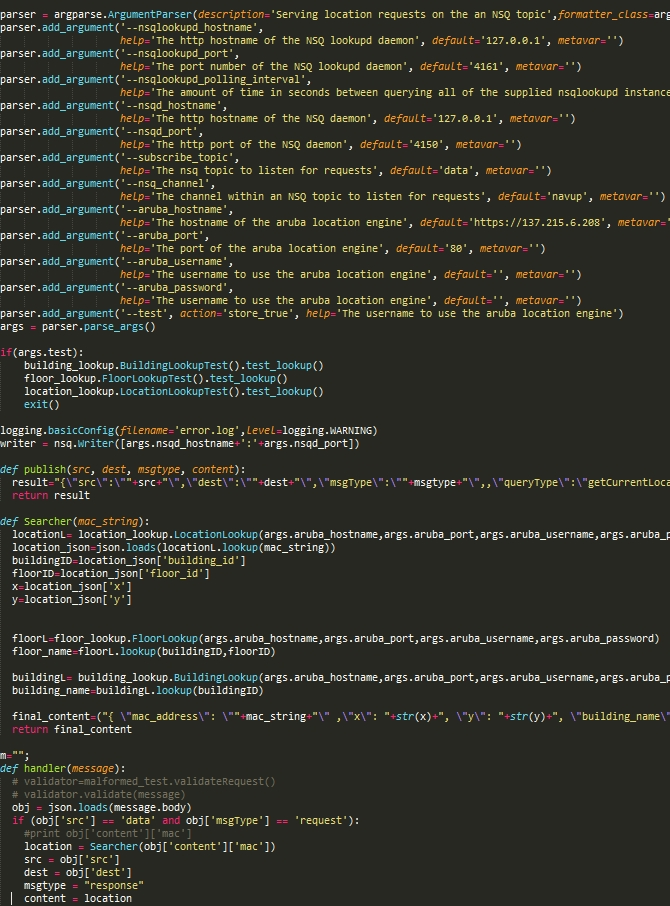
\includegraphics[width=350px]{Images/nocomments.jpg}
  \caption{No Comments}
  \label{Figure showing the lack of comments and explanation}
\end{figure}

\newpage
\newpage
\section{Use Cases}

\begin{flushleft}
Broadsword has made use of a NSQ.
A 'nsqd' instance is designed to handle multiple streams of data at once.
In NSQ terms, streams are called "topics" where a topic can have 1 or more "channels".
A channel maps to a downstream service consuming a topic.
The method broadsword used was to create a topic, "data", through subscribing to channel "navup", which is a channel on the "data" topic. The topic is created through the first subscription.
This method lets channels and topics buffer their data independently. This allows for fast downstream, preventing a slow consumer to cause a bottleneck or delay.
\bigskip

Successful upstream and downstream communication ticks the use case boxes, although more efficient changes could be made for concurrent processing, a mark of 8 out of 10 for downstream and upstream seems fair.
\end{flushleft}


\subsection{Upstream communication.}
\begin{flushleft}
MARK: 8
\end{flushleft}

\begin{flushleft}
The file named "publisher.py" will write to nsqd port 4150, this is their upstream communication channel.
\end{flushleft}


\begin{figure}[ht]
  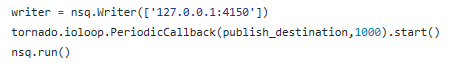
\includegraphics[width=350px]{Images/publisher.PNG}
   \caption{Upstream channel}
  \label{Upstream channel initializer}  
\end{figure}

\subsection{Downstream communication.}
\begin{flushleft}
MARK: 8
\end{flushleft}

\begin{flushleft}
Consumers make use of a HTTP /lookup endpoint. Consumers are introduced to topics through making use of the addresses of Broadsword's nsqlookupd instance. In their case it would be host name '127.0.0.1' and port '4161'. This would be their downstream communication.
\end{flushleft}


\begin{figure}[ht]
  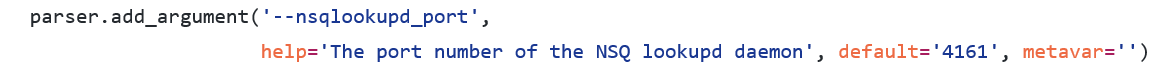
\includegraphics[width=350px]{Images/readerInitialize.PNG}
  \caption{Downstream channel initialize}
  \label{Downstream channel initializer}  
\end{figure}

\begin{figure}[ht]
  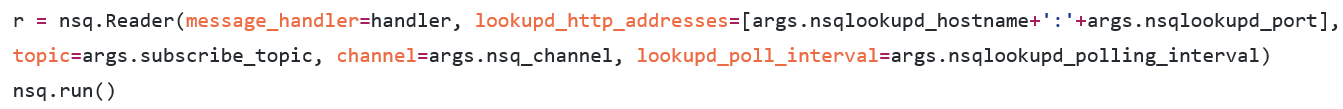
\includegraphics[width=350px]{Images/readerExecute.PNG}
  \caption{Downstream channel execute}
  \label{Downstream channel executer}  
\end{figure}

\newpage
\subsection{Security.}
\begin{flushleft}
MARK: 8
\end{flushleft}

\begin{flushleft}
Broadsword requires that the login credentials for Aruba be passed into their program via parameters rather than being specified directly in the code. This creates a layer of security as had the details been hard coded, anyone could access and discover them simply by looking at the code. This is especially true as the project is currently open source and available freely on GitHub.
\end{flushleft}

\begin{flushleft}
This was a very mindful decision on Broadswords part and a nice touch, however they do not handle an incorrect password very effectively. Having actively made the decision to pass in the details via function arguments one could expect that they would handle an incorrect password however this is not the case and this is demonstrated in the figure below. An incorrect password results in an uncaught exception in the program. This is not desirable as one cannot decipher the cause simply by examining the error message.
\end{flushleft}

\begin{figure}[ht]
  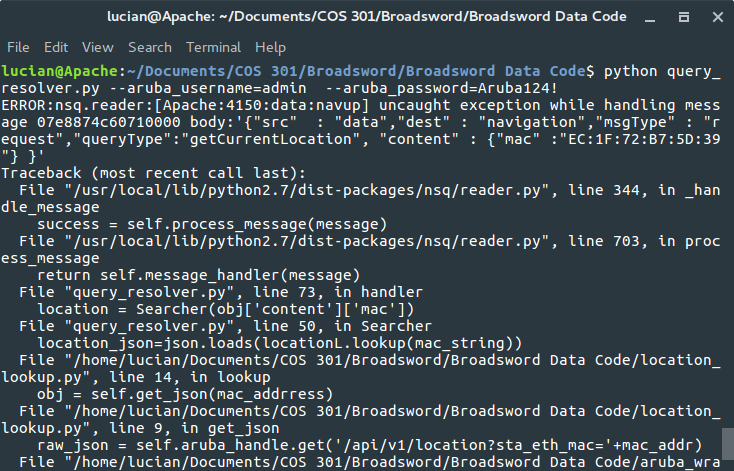
\includegraphics[width=350px]{Images/Incorrect_Password.png}
  \caption{Exception occurring when an incorrect password is used.}
  \label{Terminal output.}  
\end{figure}

\begin{flushleft}
The non-functional requirement is there however and as a result Broadsword receives the mark of 8/10 for this section.
\end{flushleft}

\section{Evaluation of Broadsword Test Cases}
\begin{flushleft}
MARK: 6
\end{flushleft}

\begin{flushleft}
The Broadsword team makes use of extensive testing cases that caver all the information necessary for the Aruba connection as well as cover the mock information For the GIS module. This good coverage provides utility for successful test cases showing results that would be used in the final NAVUP system. 
\end{flushleft}

\begin{flushleft}
The MAC address that is handed to the 'aruba\textunderscore wrapper' class, involved in the Aruba Ale connection and communication, are chosen randomly from a group of 4 available test cases. This provides some sense of variety in the testing of the system. 
\end{flushleft}

\begin{flushleft}
The issue with the current test cases is that although the coverage may seem extensive, the fulfillment of the non-functional requirement of concurrency is not tested in any form. Concurrency is an important part of the data streaming service for the final NAVUP system. In conclusion for good test-case coverage, variety in MAC address testing as well as extensive mock input data and classes whilst keeping in mind the lack of concurrency and speed and its importance to the project, a mark of 6 is given.
\end{flushleft}


\begin{figure}[ht]
  \includegraphics[width=350px]{Images/MAC.jpg}
  \caption{The random selection of MAC addresses}
  \label{The random selection of MAC addresses}  
\end{figure}

\begin{figure}[ht]
  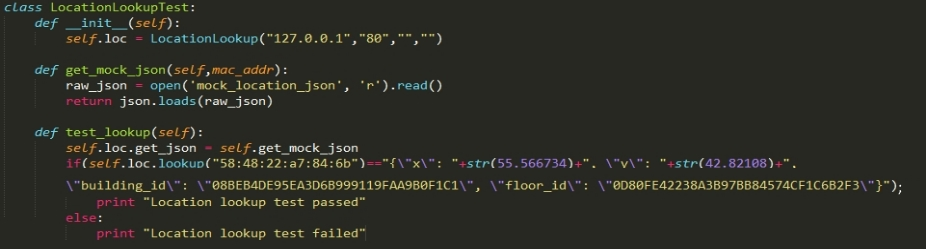
\includegraphics[width=350px]{Images/Mock.jpg}
  \caption{An image showing tests on different parts of the data system}
  \label{An image showing test date to test different part of the data system}  
\end{figure}

\section{Conclusion}
\begin{flushleft}
In conclusion, as a team we felt that the Broadsword Data team only implemented the core functionality of the module at hand and did not focus the majority of their efforts into making sure that high speed data streaming takes place at all times. This could have been misleading by the fact that requests can be issued to the NSQ Server at a very high rate, but this is merely adding to the queue and these requests are not serviced in ample time so as to serve the task at hand. 
\\
After taking into consideration all the tests performed with quantitative and qualitative data, and after critical assessment of their code, we as a team have come to a conclusion of a mark of 73/120 , which translates to a percentage of 60.8\%. 
\end{flushleft}

\end{document}
